\documentclass[10 pt,a4paper, article]{amsart}

% --------------------
% Title information
% --------------------
\title{Extracted exponents of prime numbers, for a factorial, obtained by recursive splitting of odd and even parts, coincide with Legendre's formula.}

\author{Amit Kumar\\Independent Researcher\\Bengaluru-India\\amit7urmc@gmail.com}
\usepackage[a4paper, margin=0.75in]{geometry}
\usepackage{amsfonts,amssymb,amscd,amsmath,enumerate,verbatim,calc}
\usepackage{graphicx}
\usepackage{float}
\usepackage{url}
\usepackage{xr}
\usepackage{tikz}
\usetikzlibrary{arrows}
\usetikzlibrary{positioning}
\newcommand{\floor}[1]{\left\lfloor #1 \right\rfloor}


% --------------------
% Document
% --------------------
\begin{document}
\maketitle

\bigskip
\noindent\textbf{Keywords:} Factorial, Legendre's formula, $p$-adic valuation, Recursion.

\smallskip
\noindent\textbf{AMS Subject Classification (MSC2020):} \\
\textbf{Primary:} 11A41; \textbf{Secondary:} 11A05, 11Y70, 97I20

\bigskip
\section{Abstract}
By recursively splitting the factorial of an integer $n$, we can ``peel off'' one prime number and its exponent at a time. We show algorithmic steps to achieve the same and demonstrate why the extracted exponents of prime numbers, obtained by this method, completely coincide with Legendre's formula for p-adic valuation, for all the prime numbers contained within $n$. This step-by-step decomposition allows us to revisit Legendre's formula and see its inner workings, with a fresh pedagogical approach!

\section{Introduction}
The factorial of an integer $n$ is denoted by $n!$ and is the product of all the integers from $1$ to $n$ (both inclusive). By the Fundamental Theorem of Arithmetic, any integer can be expressed as the product of its constituent prime numbers (each raised to an appropriate exponent). Furthermore, within this range, some prime numbers occur repeatedly, each with possibly different exponents. With little effort, it can be seen that the different occurrences of exponents can be combined into a single number. Thus, a factorial is simply a product of the prime numbers (not exceeding $n$) raised to their respective exponents. A natural question comes to mind: given a factorial ($n!$), can we recover the prime numbers (within $n$) and the exponents attached to them?

The nineteenth-century French Mathematician, A.M. Legendre, gave a formula to calculate the exponent for any prime number inside $n!$. This formula gives the \emph{p-adic valuation of n} and is as follows.
\begin{align*}
\nu_p(n!) &= \sum_{i=1}^{\infty} \left\lfloor \frac{n}{p^i} \right\rfloor
\end{align*}
The $\left\lfloor \frac{n}{p^i} \right\rfloor$ symbol denotes the greatest integer less than or equal to $\frac{n}{p^i}$.

e.g For $35!$, we can calculate $\nu_2(35!)$ to be as 
\begin{align*}
&= \left\lfloor \frac{35}{2^1} \right\rfloor + \left\lfloor \frac{35}{2^2} \right\rfloor + \left\lfloor \frac{35}{2^3} \right\rfloor + \left\lfloor \frac{35}{2^4} \right\rfloor + \left\lfloor \frac{35}{2^5} \right\rfloor \quad \text{...higher powers will result in 0} \\
&= \left\lfloor \frac{35}{2} \right\rfloor + \left\lfloor \frac{35}{4} \right\rfloor + \left\lfloor \frac{35}{8} \right\rfloor + \left\lfloor \frac{35}{16} \right\rfloor + \left\lfloor \frac{35}{32} \right\rfloor \\
&= 17 + 8 + 4 + 2 + 1 \\
&= 32
\end{align*}

For $35!$, we can calculate $\nu_3(35!)$ to be as 
\begin{align*}
&= \left\lfloor \frac{35}{3^1} \right\rfloor + \left\lfloor \frac{35}{3^2} \right\rfloor + \left\lfloor \frac{35}{3^3} \right\rfloor \text{...higher powers will result in 0, so dropped} \\
&= \left\lfloor \frac{35}{3} \right\rfloor + \left\lfloor \frac{35}{9} \right\rfloor + \left\lfloor \frac{35}{27} \right\rfloor \\
&= 11 + 3 + 1 \\
&= 15
\end{align*}
We can continue this process until all prime numbers are covered. Continuing beyond that will only yield 0 (due to floor division). To make full use of Legendre's formula, one needs to know all the prime numbers in advance (by a suitable method grounded in number theory).

The purpose of this article is to show that using a simple-to-follow algorithmic steps, it is possible to recover both: the prime numbers contained within $n$ and the respective exponent of each prime number. We started by asking if the factorial of an integer has any underlying structure. In this pursuit, we split the full factorial into two parts: one with all odd numbers and one with all even numbers. We immediately saw recursion emerging (with particular focus on the even part). While we work through the recursive structure of the even part, the odd numbers keep accumulating in the other half. At the end of the recursion, when we look at the ``assembled" odd integers, an elegant underlying structure of prime numbers comes to the fore. From this structure, we can peel off the prime number with its exponent, one layer at a time. The total exponent retrieved for each prime agrees exactly with \emph{Legendre's p-adic valuation}. This agreement between two independently developed ideas - recursive decomposition of the factorial structure and \emph{Legendre's p-adic valuation} - allows us to revisit \emph{Legendre's p-adic valuation} with a new pedagogical approach. 

It is interesting to see the inner machinery of \emph{Legendre's p-adic valuation} when the steps suggested in this article are followed. At the end of the process, the entire factorial is decomposed into the constituent prime numbers raised to appropriate exponents. The ``peeling off, of layers of prime numbers" stops early, and the recursive decomposition is complete. At that time, the algorithm halts! At the end, we have decomposed the factorial of $n$, ($n!$), into the prime numbers and their exponents, yet stay in harmony with \emph{Legendre's p-adic valuation}, using a single algorithm.

\section{Main content}\label{sec:maincontent}

\subsection{Recursive decomposition of the factorial.}
Let us see how the recursion emerges in a factorial. We will take a concrete example of $35!$:
\begin{align*}
35! &= 1 \times 2 \times 3 \cdots \times 33 \times 34 \times 35 \\
    &= (1 \times 3 \times 5 \cdots \times 31 \times 33 \times 35) \times (2 \times 4 \times 6 \times \cdots \times 30 \times 32 \times 34) \\
    \intertext{factor 2 out from the right bracket}
    &= (1 \times 3 \times 5 \cdots \times 31 \times 33 \times 35) \times 2^{17} \times (1 \times 2 \times 3 \times \cdots \times 16 \times 17) \\
    &= (1 \times 3 \times 5 \cdots \times 33 \times 35) \times 2^{17} \times (1 \times 3 \cdots \times 17) \times (2 \times 4 \times \cdots \times 16) \\
    &= (\text{all odd products}) \times 2^{17} \times 2^8 \times (1 \times 2 \times 3 \times \cdots \times 6 \times 7 \times 8) \\
    &= (\text{all odd products}) \times 2^{17} \times 2^8 \times 2^4 \times (1 \times 2 \times 3 \times 4) \\
    &= (\text{all odd products}) \times 2^{17} \times 2^8 \times 2^4 \times 2^2 \times (1 \times 2) \\
    &= (\text{all odd products}) \times 2^{17} \times 2^8 \times 2^4 \times 2^2 \times 2^1 \times 1 \\
    &= \text{(stopping here since $1$ cannot be factored further)}
\end{align*}
Please notice that while we peeled off the contribution of the prime number $2$ from the factorial, at every step we removed the exponents in perfect agreement with \emph{Legendre's p-adic valuation for prime $2$}.

While there is only a single even prime, $2$, there are an infinite number of primes that are odd. While we were focusing on prime $2$, the odd numbers were, naturally, accumulating in the other half (see below). These odd parts have all the remaining prime numbers and exponents present in an encoded way. We need to recover them! 
\begin{align*}
35! = {2^{32}}\times(1 \times 3 \times 5 \times 7 \times 9 \times 11 \times 13 \times 15 \times 17 \times 19 \cdots 31 \times 33 \times 35) \times \\
(1 \times 3 \times 5 \times 7 \times 9 \times 11 \times 13 \times 15 \times 17) \times \\
(1 \times 3 \times 5 \times 7) \times \\
(1 \times 3) \\
.
\end{align*} 
Although we appreciate some pattern above, at this stage it is not yet obvious how to proceed! We start by observing that we can combine powers of each number and arrange the numbers in a sorted order from left to right. This gives a unified arrangement as follows:
\begin{multline*}
35! = {2^{32}} \times (1 \times 3^{4} \times 5^{3} \times 7^{3} \times 9^2 \times 11^2 \times 13^2 \times 15^2 \times 17^2 \times 19 \times 21 \times 23 \\
\times 25 \times 27 \times 29 \times 31 \times 33 \times 35)
\end{multline*}

Now we make another observation that all the multiples of prime $3$ are $3$ steps apart, all the multiples of $5$ are $5$ steps apart and so on (Figure \ref{fig:hop-3}). We can safely introduce two steps: `hop' and `collect'! We `hop' $x$ steps on the remaining/rearranged number line, whereby we are guaranteed to land on the multiples of $x$. We `collect' exponents from each slot and add to the grand total for the prime number `$x$'. At the end of the `hop and collect' step for the prime, all the contributions of the prime $x$ are guranteed to have been ``peeled off" from every number to its right. This will not only result in the decomposition of any odd number (on the right) but is also guaranteed to reveal the next prime number (after discarding the number $1$). It is easy to see that we repeat this process until we cannot `hop' anymore, since we will land outside the right boundary of the arrangement of numbers.

As per the above algorithm, we start the process with prime $3$ and thus we have to `hop and collect' all powers of $3$ present at each slot (Figure \ref{fig:collect-3}).

\begin{figure}[htbp]
    \centering
    \resizebox{\textwidth}{!}{%
	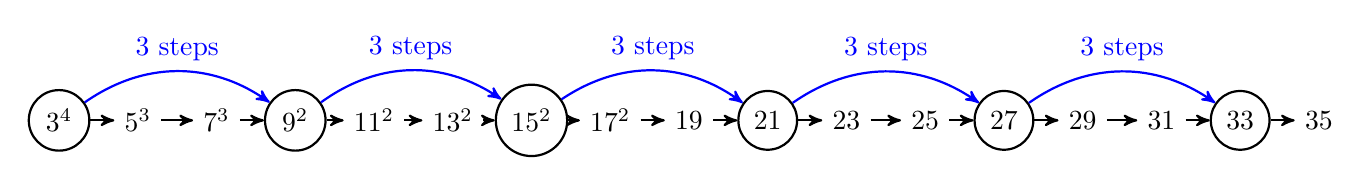
\begin{tikzpicture}[
		->,
		>=stealth',
		auto,
		node distance=1.0cm,
		thick,
		main node/.style={font=\sffamily\bfseries}
		,
		circled node/.style={
			main node,
			circle,
			draw
		}
		]
		
		\node[circled node] (n1) {$3^{4}$};
		\node[main node] (n2) [right of=n1] {$5^{3}$};
		\node[main node] (n3) [right of=n2] {$7^{3}$};
		\node[circled node] (n4) [right of=n3] {$9^{2}$};
		\node[main node] (n5) [right of=n4] {$11^{2}$};
		\node[main node] (n6) [right of=n5] {$13^{2}$};
		\node[circled node] (n7) [right of=n6] {$15^{2}$};
		\node[main node] (n8) [right of=n7] {$17^{2}$};
		\node[main node] (n9) [right of=n8] {$19$};
		\node[circled node] (n10) [right of=n9] {$21$};
		\node[main node] (n11) [right of=n10] {$23$};
		\node[main node] (n12) [right of=n11] {$25$};
		\node[circled node] (n13) [right of=n12] {$27$};
		\node[main node] (n14) [right of=n13] {$29$};
		\node[main node] (n15) [right of=n14] {$31$};
		\node[circled node] (n16) [right of=n15] {$33$};
		\node[main node] (n17) [right of=n16] {$35$};
		
		\path
		(n1) edge (n2)
		(n2) edge (n3)
		(n3) edge (n4)
		(n4) edge (n5)
		(n5) edge (n6)
		(n6) edge (n7)
		(n7) edge (n8)
		(n8) edge (n9)
		(n9) edge (n10)
		(n10) edge (n11)
		(n11) edge (n12)
		(n12) edge (n13)
		(n13) edge (n14)
		(n14) edge (n15)
		(n15) edge (n16)
		(n16) edge (n17);
		\draw[->, thick, blue, bend left=35] (n1) to node[midway, above, blue] {3 steps} (n4);
		\draw[->, thick, blue, bend left=35] (n4) to node[midway, above, blue] {3 steps} (n7);
		\draw[->, thick, blue, bend left=35] (n7) to node[midway, above, blue] {3 steps} (n10);
		\draw[->, thick, blue, bend left=35] (n10) to node[midway, above, blue] {3 steps} (n13);
		\draw[->, thick, blue, bend left=35] (n13) to node[midway, above, blue] {3 steps} (n16);
	\end{tikzpicture}\newline
    }
    \caption{Hop-step for prime 3}
    \label{fig:hop-3}
\end{figure}

\begin{figure}[htbp]
    \centering
    \resizebox{\textwidth}{!}{%
	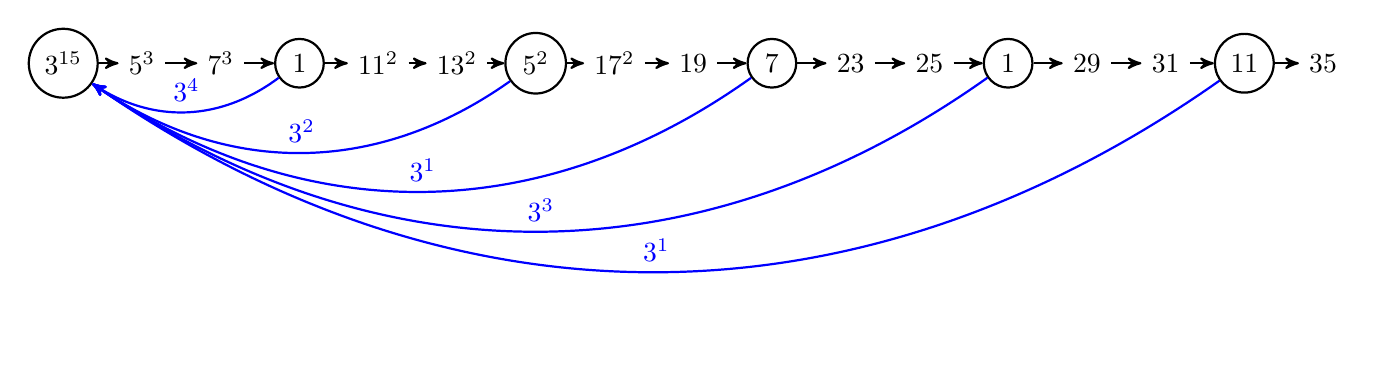
\begin{tikzpicture}[
		->,
		>=stealth',
		auto,
		node distance=1.0cm,
		thick,
		main node/.style={font=\sffamily\bfseries}
		,
		circled node/.style={
			main node,
			circle,
			draw
		}
		]
		
		\node[circled node] (n1) {$3^{15}$};
		\node[main node] (n2) [right of=n1] {$5^{3}$};
		\node[main node] (n3) [right of=n2] {$7^{3}$};
		\node[circled node] (n4) [right of=n3] {$1$};
		\node[main node] (n5) [right of=n4] {$11^{2}$};
		\node[main node] (n6) [right of=n5] {$13^{2}$};
		\node[circled node] (n7) [right of=n6] {$5^{2}$};
		\node[main node] (n8) [right of=n7] {$17^{2}$};
		\node[main node] (n9) [right of=n8] {$19$};
		\node[circled node] (n10) [right of=n9] {$7$};
		\node[main node] (n11) [right of=n10] {$23$};
		\node[main node] (n12) [right of=n11] {$25$};
		\node[circled node] (n13) [right of=n12] {$1$};
		\node[main node] (n14) [right of=n13] {$29$};
		\node[main node] (n15) [right of=n14] {$31$};
		\node[circled node] (n16) [right of=n15] {$11$};
		\node[main node] (n17) [right of=n16] {$35$};
		
		\path
		(n1) edge (n2)
		(n2) edge (n3)
		(n3) edge (n4)
		(n4) edge (n5)
		(n5) edge (n6)
		(n6) edge (n7)
		(n7) edge (n8)
		(n8) edge (n9)
		(n9) edge (n10)
		(n10) edge (n11)
		(n11) edge (n12)
		(n12) edge (n13)
		(n13) edge (n14)
		(n14) edge (n15)
		(n15) edge (n16)
		(n16) edge (n17);
		\draw[->, thick, blue, bend left=35] (n4) to node[midway, above, blue] {$3^{4}$} (n1);
		\draw[->, thick, blue, bend left=35] (n7) to node[midway, above, blue] {$3^{2}$} (n1);
		\draw[->, thick, blue, bend left=35] (n10) to node[midway, above, blue] {$3^{1}$} (n1);
		\draw[->, thick, blue, bend left=35] (n13) to node[midway, above, blue] {$3^{3}$} (n1);
		\draw[->, thick, blue, bend left=35] (n16) to node[midway, above, blue] {$3^{1}$} (n1);
	\end{tikzpicture}
    }
    \caption{Collect step for prime 3}
    \label{fig:collect-3}
\end{figure}



	
After collect step of prime number $3$, we remove the $3$ with its exponent from the front of the queue. We shift our attention to the next number in the queue, which is not equal to $1$ (in this case, $5$). It is easy to see that once the previous number has been removed, the number remaining in the front of the queue is the next prime number [since it could not be collected in any of the previous steps]. As observed before, the slots are again $5$ units apart. 

We repeat the same process for $5$: hopping 5 steps at a time (Figure \ref{fig:hop-5}) and remove and collect the highest power of $5$ at every step as below (Figure \ref{fig:collect-5}).\newline

\begin{figure}[htbp]
    \centering
    \resizebox{\textwidth}{!}{%
	\begin{tikzpicture}[
		->,
		>=stealth',
		auto,
		node distance=1.0cm,
		thick,
		main node/.style={font=\sffamily\bfseries}
		,
		circled node/.style={
			main node,
			circle,
			draw
		}
		]
		
		\node[circled node] (n2) [right of=n1] {$5^{3}$};
		\node[main node] (n3) [right of=n2] {$7^{3}$};
		\node[main node] (n4) [right of=n3] {$1$};
		\node[main node] (n5) [right of=n4] {$11^{2}$};
		\node[main node] (n6) [right of=n5] {$13^{2}$};
		\node[circled node] (n7) [right of=n6] {$5^{2}$};
		\node[main node] (n8) [right of=n7] {$17^{2}$};
		\node[main node] (n9) [right of=n8] {$19$};
		\node[main node] (n10) [right of=n9] {$7$};
		\node[main node] (n11) [right of=n10] {$23$};
		\node[circled node] (n12) [right of=n11] {$25$};
		\node[main node] (n13) [right of=n12] {$1$};
		\node[main node] (n14) [right of=n13] {$29$};
		\node[main node] (n15) [right of=n14] {$31$};
		\node[main node] (n16) [right of=n15] {$11$};
		\node[circled node] (n17) [right of=n16] {$35$};
		
		\path
		(n2) edge (n3)
		(n3) edge (n4)
		(n4) edge (n5)
		(n5) edge (n6)
		(n6) edge (n7)
		(n7) edge (n8)
		(n8) edge (n9)
		(n9) edge (n10)
		(n10) edge (n11)
		(n11) edge (n12)
		(n12) edge (n13)
		(n13) edge (n14)
		(n14) edge (n15)
		(n15) edge (n16)
		(n16) edge (n17);
		\draw[->, thick, blue, bend left=35] (n2) to node[midway, above, blue] {5 steps} (n7);
		\draw[->, thick, blue, bend left=35] (n7) to node[midway, above, blue] {5 steps} (n12);
		\draw[->, thick, blue, bend left=35] (n12) to node[midway, above, blue] {5 steps} (n17);
	\end{tikzpicture}
    }
    \caption{Hop-step for prime 5}
    \label{fig:hop-5}
\end{figure}
	
	

\begin{figure}[htbp]
    \centering
    \resizebox{\textwidth}{!}{%
	\begin{tikzpicture}[
		->,
		>=stealth',
		auto,
		node distance=1.0cm,
		thick,
		main node/.style={font=\sffamily\bfseries}
		,
		circled node/.style={
			main node,
			circle,
			draw
		}
		]
		
		\node[circled node] (n2) [right of=n1] {$5^{8}$};
		\node[main node] (n3) [right of=n2] {$7^{3}$};
		\node[main node] (n4) [right of=n3] {$1$};
		\node[main node] (n5) [right of=n4] {$11^{2}$};
		\node[main node] (n6) [right of=n5] {$13^{2}$};
		\node[circled node] (n7) [right of=n6] {$1$};
		\node[main node] (n8) [right of=n7] {$17^{2}$};
		\node[main node] (n9) [right of=n8] {$19$};
		\node[main node] (n10) [right of=n9] {$7$};
		\node[main node] (n11) [right of=n10] {$23$};
		\node[circled node] (n12) [right of=n11] {$1$};
		\node[main node] (n13) [right of=n12] {$1$};
		\node[main node] (n14) [right of=n13] {$29$};
		\node[main node] (n15) [right of=n14] {$31$};
		\node[main node] (n16) [right of=n15] {$11$};
		\node[circled node] (n17) [right of=n16] {$7$};
		
		\path
		(n2) edge (n3)
		(n3) edge (n4)
		(n4) edge (n5)
		(n5) edge (n6)
		(n6) edge (n7)
		(n7) edge (n8)
		(n8) edge (n9)
		(n9) edge (n10)
		(n10) edge (n11)
		(n11) edge (n12)
		(n12) edge (n13)
		(n13) edge (n14)
		(n14) edge (n15)
		(n15) edge (n16)
		(n16) edge (n17);
		\draw[->, thick, blue, bend left=35] (n7) to node[midway, above, blue] {$5^{2}$} (n2);
		\draw[->, thick, blue, bend left=35] (n12) to node[midway, above, blue] {$5^{2}$} (n2);
		\draw[->, thick, blue, bend left=35] (n17) to node[midway, above, blue] {$5^{1}$} (n2);
	\end{tikzpicture}
    }
    \caption{Collect step for prime 5}
    \label{fig:collect-5}
\end{figure}


	
	The process is repeated for the next exposed number at the front of the queue: $7$ (by jumping 7 units and extracting/collecting the highest power of 7 at each step: Figures \ref{fig:hop-7} and \ref{fig:collect-7}). \newline

\begin{figure}[htbp]
    \centering
    \resizebox{\textwidth}{!}{%
	\begin{tikzpicture}[
		->,
		>=stealth',
		auto,
		node distance=1.0cm,
		thick,
		main node/.style={font=\sffamily\bfseries}
		,
		circled node/.style={
			main node,
			circle,
			draw
		}
		]
		\node[circled node] (n3) [right of=n2] {$7^{3}$};
		\node[main node] (n4) [right of=n3] {$1$};
		\node[main node] (n5) [right of=n4] {$11^{2}$};
		\node[main node] (n6) [right of=n5] {$13^{2}$};
		\node[main node] (n7) [right of=n6] {$1$};
		\node[main node] (n8) [right of=n7] {$17^{2}$};
		\node[main node] (n9) [right of=n8] {$19$};
		\node[circled node] (n10) [right of=n9] {$7$};
		\node[main node] (n11) [right of=n10] {$23$};
		\node[main node] (n12) [right of=n11] {$1$};
		\node[main node] (n13) [right of=n12] {$1$};
		\node[main node] (n14) [right of=n13] {$29$};
		\node[main node] (n15) [right of=n14] {$31$};
		\node[main node] (n16) [right of=n15] {$11$};
		\node[circled node] (n17) [right of=n16] {$7$};
		
		\path
		(n3) edge (n4)
		(n4) edge (n5)
		(n5) edge (n6)
		(n6) edge (n7)
		(n7) edge (n8)
		(n8) edge (n9)
		(n9) edge (n10)
		(n10) edge (n11)
		(n11) edge (n12)
		(n12) edge (n13)
		(n13) edge (n14)
		(n14) edge (n15)
		(n15) edge (n16)
		(n16) edge (n17);
		\draw[->, thick, blue, bend left=35] (n3) to node[midway, above, blue] {7 steps} (n10);
		\draw[->, thick, blue, bend left=35] (n10) to node[midway, above, blue] {7 steps} (n17);
	\end{tikzpicture}
    }
    \caption{Hop-step for prime 7}
    \label{fig:hop-7}
\end{figure}

	
\begin{figure}[htbp]
    \centering
    \resizebox{\textwidth}{!}{%
		\begin{tikzpicture}[
		->,
		>=stealth',
		auto,
		node distance=1.0cm,
		thick,
		main node/.style={font=\sffamily\bfseries}
		,
		circled node/.style={
			main node,
			circle,
			draw
		}
		]
		\node[circled node] (n3) [right of=n2] {$7^{5}$};
		\node[main node] (n4) [right of=n3] {$1$};
		\node[main node] (n5) [right of=n4] {$11^{2}$};
		\node[main node] (n6) [right of=n5] {$13^{2}$};
		\node[main node] (n7) [right of=n6] {$1$};
		\node[main node] (n8) [right of=n7] {$17^{2}$};
		\node[main node] (n9) [right of=n8] {$19$};
		\node[circled node] (n10) [right of=n9] {$1$};
		\node[main node] (n11) [right of=n10] {$23$};
		\node[main node] (n12) [right of=n11] {$1$};
		\node[main node] (n13) [right of=n12] {$1$};
		\node[main node] (n14) [right of=n13] {$29$};
		\node[main node] (n15) [right of=n14] {$31$};
		\node[main node] (n16) [right of=n15] {$11$};
		\node[circled node] (n17) [right of=n16] {$1$};
		
		\path
		(n3) edge (n4)
		(n4) edge (n5)
		(n5) edge (n6)
		(n6) edge (n7)
		(n7) edge (n8)
		(n8) edge (n9)
		(n9) edge (n10)
		(n10) edge (n11)
		(n11) edge (n12)
		(n12) edge (n13)
		(n13) edge (n14)
		(n14) edge (n15)
		(n15) edge (n16)
		(n16) edge (n17);
		\draw[->, thick, blue, bend left=35] (n10) to node[midway, above, blue] {$7^{1}$} (n3);
		\draw[->, thick, blue, bend left=35] (n17) to node[midway, above, blue] {$7^{1}$} (n3);
	\end{tikzpicture}\newline
    }
    \caption{Collect step for prime 7}
    \label{fig:collect-7}
\end{figure}	

	
	We continue to the next prime (skipping 1), which is $11$ and repeat the hop and collect steps (Figures \ref{fig:hop-11} and \ref{fig:collect-11}).\newline
	
\begin{figure}[htbp]
    \centering
    \resizebox{\textwidth}{!}{%
		\begin{tikzpicture}[
		->,
		>=stealth',
		auto,
		node distance=1.0cm,
		thick,
		main node/.style={font=\sffamily\bfseries}
		,
		circled node/.style={
			main node,
			circle,
			draw
		}
		];
		\node[circled node] (n5) [right of=n4] {$11^{2}$};
		\node[main node] (n6) [right of=n5] {$13^{2}$};
		\node[main node] (n7) [right of=n6] {$1$};
		\node[main node] (n8) [right of=n7] {$17^{2}$};
		\node[main node] (n9) [right of=n8] {$19$};
		\node[main node] (n10) [right of=n9] {$1$};
		\node[main node] (n11) [right of=n10] {$23$};
		\node[main node] (n12) [right of=n11] {$1$};
		\node[main node] (n13) [right of=n12] {$1$};
		\node[main node] (n14) [right of=n13] {$29$};
		\node[main node] (n15) [right of=n14] {$31$};
		\node[circled node] (n16) [right of=n15] {$11$};
		\node[main node] (n17) [right of=n16] {$1$};
		
		\path
		(n5) edge (n6)
		(n6) edge (n7)
		(n7) edge (n8)
		(n8) edge (n9)
		(n9) edge (n10)
		(n10) edge (n11)
		(n11) edge (n12)
		(n12) edge (n13)
		(n13) edge (n14)
		(n14) edge (n15)
		(n15) edge (n16)
		(n16) edge (n17);
		\draw[->, thick, blue, bend left=35] (n5) to node[midway, above, blue] {11 steps} (n16);
	\end{tikzpicture}
    }
    \caption{Hop-step for prime 11.}
    \label{fig:hop-11}
\end{figure}	

\begin{figure}[htbp]
    \centering
    \resizebox{\textwidth}{!}{%
	\begin{tikzpicture}[
		->,
		>=stealth',
		auto,
		node distance=1.0cm,
		thick,
		main node/.style={font=\sffamily\bfseries}
		,
		circled node/.style={
			main node,
			circle,
			draw
		}
		];
		\node[circled node] (n5) [right of=n4] {$11^{3}$};
		\node[main node] (n6) [right of=n5] {$13^{2}$};
		\node[main node] (n7) [right of=n6] {$1$};
		\node[main node] (n8) [right of=n7] {$17^{2}$};
		\node[main node] (n9) [right of=n8] {$19$};
		\node[main node] (n10) [right of=n9] {$1$};
		\node[main node] (n11) [right of=n10] {$23$};
		\node[main node] (n12) [right of=n11] {$1$};
		\node[main node] (n13) [right of=n12] {$1$};
		\node[main node] (n14) [right of=n13] {$29$};
		\node[main node] (n15) [right of=n14] {$31$};
		\node[circled node] (n16) [right of=n15] {$1$};
		\node[main node] (n17) [right of=n16] {$1$};
		
		\path
		(n5) edge (n6)
		(n6) edge (n7)
		(n7) edge (n8)
		(n8) edge (n9)
		(n9) edge (n10)
		(n10) edge (n11)
		(n11) edge (n12)
		(n12) edge (n13)
		(n13) edge (n14)
		(n14) edge (n15)
		(n15) edge (n16)
		(n16) edge (n17);
		\draw[->, thick, blue, bend left=35] (n16) to node[midway, above, blue] {$11^{1}$} (n5);
	\end{tikzpicture}
    }
    \caption{Collect step for prime 11.}
    \label{fig:collect-11}
\end{figure}	

	
	This brings us to the last step and the prime number $13$. We do not need to continue beyond this since the next hop of 13 is outside the last number slot on the right of the queue, \textit{i.e. $n$} (Figure \ref{fig:lastStep}). Interestingly, the decomposition process is also complete at the same time, such that the remaining numbers are either prime (raised to respective exponents) or 1. The algorithm stops here, and no further ``peeling off" is required! \newline
	
\begin{figure}[htbp]
    \centering
    \resizebox{\textwidth}{!}{%
	\begin{tikzpicture}[
		->,
		>=stealth',
		auto,
		node distance=1.0cm,
		thick,
		main node/.style={font=\sffamily\bfseries}
		,
		circled node/.style={
			main node,
			circle,
			draw
		}
		]
		\node[circled node] (n6) [right of=n5] {$13^{2}$};
		\node[main node] (n7) [right of=n6] {$1$};
		\node[main node] (n8) [right of=n7] {$17^{2}$};
		\node[main node] (n9) [right of=n8] {$19$};
		\node[main node] (n10) [right of=n9] {$1$};
		\node[main node] (n11) [right of=n10] {$23$};
		\node[main node] (n12) [right of=n11] {$1$};
		\node[main node] (n13) [right of=n12] {$1$};
		\node[main node] (n14) [right of=n13] {$29$};
		\node[main node] (n15) [right of=n14] {$31$};
		\node[main node] (n16) [right of=n15] {$1$};
		\node[main node] (n17) [right of=n16] {$1$};
		\node[circled node] (n18) [right of=n17] {X};
		
		\path
		(n6) edge (n7)
		(n7) edge (n8)
		(n8) edge (n9)
		(n9) edge (n10)
		(n10) edge (n11)
		(n11) edge (n12)
		(n12) edge (n13)
		(n13) edge (n14)
		(n14) edge (n15)
		(n15) edge (n16)
		(n16) edge (n17);
		\draw[->, dashed, red, bend left=35] (n6) to node[midway, above, blue] {Invalid step. Abort!} (n18);
	\end{tikzpicture}
    }
    \caption{Last step - hopping lands beyond the right of the queue}
    \label{fig:lastStep}
\end{figure}	

	
	Thus, we have extracted all the prime numbers and their powers, after discarding the number $1$ (see below)! Each prime and its exponent is in perfect agreement with Legendre's formula for $35!$ (Figure \ref{fig:agreementWithLegendre}). \newline
\begin{figure}[htbp]
    \centering
    \resizebox{\textwidth}{!}{%
	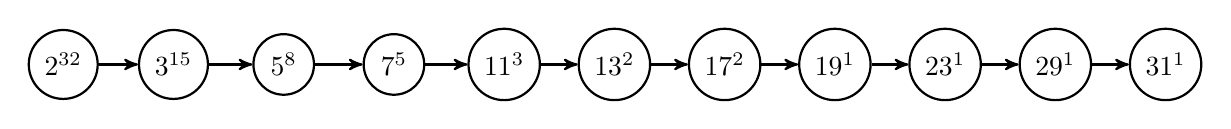
\begin{tikzpicture}[
		->,
		>=stealth',
		auto,
		node distance=1.4cm,
		thick,
		main node/.style={font=\sffamily\bfseries}
		,
		circled node/.style={
			main node,
			circle,
			draw
		}
		]
		\node[circled node] (n2) {$2^{32}$};
		\node[circled node] (n3) [right of=n2] {$3^{15}$};
		\node[circled node] (n5) [right of=n3] {$5^{8}$};
		\node[circled node] (n7) [right of=n5] {$7^{5}$};
		\node[circled node] (n11) [right of=n7] {$11^{3}$};
		\node[circled node] (n13) [right of=n11] {$13^{2}$};
		\node[circled node] (n17) [right of=n13] {$17^{2}$};
		\node[circled node] (n19) [right of=n17] {$19^{1}$};
		\node[circled node] (n23) [right of=n19] {$23^{1}$};
		\node[circled node] (n29) [right of=n23] {$29^1$};
		\node[circled node] (n31) [right of=n29] {$31^{1}$};
		
		\path
		(n2) edge (n3)
		(n3) edge (n5)
		(n5) edge (n7)
		(n7) edge (n11)
		(n11) edge (n13)
		(n13) edge (n17)
		(n17) edge (n19)
		(n19) edge (n23)
		(n23) edge (n29)
		(n29) edge (n31);
	\end{tikzpicture}
    }
    \caption{The final factorial decomposed into prime numbers with their exponents}
    \label{fig:agreementWithLegendre}
\end{figure}	
	
Multiplying all the prime numbers with their coefficients gives \\ $10333147966386144929666651337523200000000$, which is exactly the value of $35!$

\subsection{Algorithm}
\begin{enumerate}
	\item \textbf{[Odd/Even split to get all powers of $2$]} Split the factorial of $n$ into odd and even parts repeatedly to extract all the powers of 2 and separate the odd part.
	\item \textbf{[Arrange the odd numbers in order]} Collect all the powers of every odd number and ensure that the odd numbers are in ascending order.
	\item \textbf{[Identify the next prime and all slots of its multiples]} Start with the left-most prime number (by keeping the left most pointer here), say $p$. Its various terms are going to be at integer steps of $p$ in the context of the above structure. Thus, terms of $p$ are going to be at  $1.p$, $2.p$, $3.p$ \dots  on the remaining arranged numbers .\label{item:SlotIdentification}
	\item \textbf{[Find exponents at each slot]} At each of the above slots (for any prime number $p$), keep extracting exponents until valid for that slot and add all the collected exponents to the total exponents of prime $p$. This will give the exponent of $p$ at that slot. Once done, go to the next slot until all eligible slots for the current prime, $p$, are done. This is guaranteed to remove the prime number's ($x$) contributions. So pure powers of $p$ will become $1$, and from the composite numbers, the prime number's contributions are automatically removed.\label{item:ExponentsRemoval}
	\item \textbf{[Repeat until valid]} At this point, move the pointer to the next prime number (must be greater than 1). Repeat steps \ref{item:SlotIdentification} to \ref{item:ExponentsRemoval} until we reach a prime number, all the multiples of which land outside the structure. By the time we reach the final prime, $p > \floor{\frac{n}{3}}$ or earlier (see Discussion), all terms have already been reduced to either 1 or their respective prime powers, demonstrating the efficiency of the 'peeling off' process.
	\item \textbf{[Multiply to get the factorial]} At this point, only prime numbers will remain (after discarding $1$) with their exponents. If we wanted to, we could multiply the prime numbers raised to the respective exponents to get the full factorial.
\end{enumerate}
	
\section{Discussion}\label{sec:discussion}
We demonstrated that using recursive decomposition, we can extract the prime numbers and their exponents contained within $n!$. Furthermore, the prime numbers and the exponents retrieved are in agreement with  Legendre's formula. Viewed in this way, Legendre's formula is no longer merely a summation formula; it emerges naturally from the recursive decomposition of the factorial. We also show that this algorithm does not visit (`peel off') all prime numbers contained within $n$, and the process tends to complete at the value when the prime $p$ becomes larger than $\floor{\frac{n}{3}}$, when $n$ becomes very large (Please see supplementary material).

\section{Acknowledgment}
After the inception of the idea and manually confirming the calculations, the recursion for the even part was discussed at math-stackexchange \url{https://math.stackexchange.com/questions/5119239/simpler-expression-sought-for-this-recursive-structure}. I am very grateful to `Dermot Craddock \url{https://math.stackexchange.com/users/1629362/dermot-craddock}' for the helpful comments.

\section{Conflict of Interest}

The author declares that there is no conflict of interest regarding the publication of this paper.

\section{Data availability}
		
Please see the supplementary material for the Python implementation of the algorithm. The Python program generated factorial for [1, 2, 3, 4, 5, 7, 9, 11, 15, 19, 29, 35, 43, 50,  101, 251, 500, 1013, 2003, 4001, 10009, 16067, 25000, 50021, 64000, 100003, 126719, 250000, 500057, 750019, 1000000], using classical iterative methods and by recursive decomposition method. For each value of N, the last stopping prime was saved. To shed more light on the relationship between log(N) and the stopping prime, a plot was generated. The Python program and the produced Excel files have been shared as supplementary materials. Beyond this, no data was generated or utilized and is therefore not mentioned. The materials can be accessed under a CC0 open-source license.

\section{Funding} 

This research received no specific grant from any funding agency in the public, commercial, or not-for-profit sectors. The author conducted this work as an independent researcher.

\section{Conflict of Interest}

The author declares no competing interests or conflicts of interest regarding the publication of this manuscript.

\begin{thebibliography}{10}
\bibitem{Legendre}
Legendre, A. M. (1830)
\newblock Théorie des Nombre
\newblock Paris: Firmin Didot Frères
\emph{Google Books},
\url{https://www.google.co.in/books/edition/Th%C3%A9orie_des_nombres/oPZRAAAAcAAJ?hl=en}.

\end{thebibliography}
\end{document}
